\chapter{Projeto Conceitual do Produto}

\section{Características gerais}

\textcolor{red}{Descrever produto de forma geral. Apresentar itens teóricos sobre o projeto a serem aprofundados ou detalhados oportunamente.}

\textcolor{red}{Apresentar e explicar a Estrutura Analítica do Projeto (EAP), tomando cuidado com a legibilidade da imagem. Se necessário, coloque a EAP dentro do comando ``\textsf{\textbackslash begin\{landscape\} \textbackslash end\{landscape\}}'' para que ela seja apresentada em uma página deitada.}

\section{Estrutura}

\textcolor{red}{Apresentar desenho em CAD, indicar dimensões por lado/aresta/cota, indicar materiais utilizados e explicar o desenho e as decisões de projeto.}

\section{Descrição de \textit{hardware}}

\textcolor{red}{A descrição de \textit{hardware} no documento deve permitir que outras pessoas repliquem o produto proposto neste documento. Para isso, deve-se explicar de forma textual os principais sub-sistemas e as escolhas de projeto, além de indicar:}

\begin{itemize}
    \item \textcolor{red}{ O diagrama de blocos \cite{blockdiagram}, que oferece uma visão geral do hardware, com as principais partes do sistema e as ligações entre elas.}
    %\item A lista de materiais \cite{bom}, que facilita a montagem do sistema, indicando tudo que deve ser adquirido. Aproveitem a lista de materiais para apresentarem o orçamento dos mesmos.
    \item \textcolor{red}{ O esquemático \cite{esquematico}, que mostra as conexões elétricas entre os componentes. Deve-se indicar os componentes por nomes e símbolos, e as conexões entre eles, incluindo a pinagem dos componentes. Se o esquemático ficar muito grande, pode-se separa-lo em vários esquemáticos. A ligação em \textit{protoboard} não é considerada um esquemático adequado.}
\end{itemize}

\textcolor{red}{A Fig. \ref{fig:diagrama_blocos_e_esquematico} apresenta o diagrama de blocos e o esquemático de um circuito conversor de corrente alternada para corrente direta, a título de exemplo. Repare que o diagrama de blocos indica os subsistemas do circuito completo apresentado no esquemático.
% Comecem com o diagrama de blocos, que é mais genérico, e depois indiquem os detalhes com a lista de materiais e os esquemáticos.
}

\begin{figure}
    \centering
    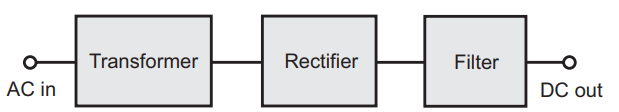
\includegraphics[width=0.5\linewidth]{figuras/Exemplo-diagrama-de-blocos.png}
    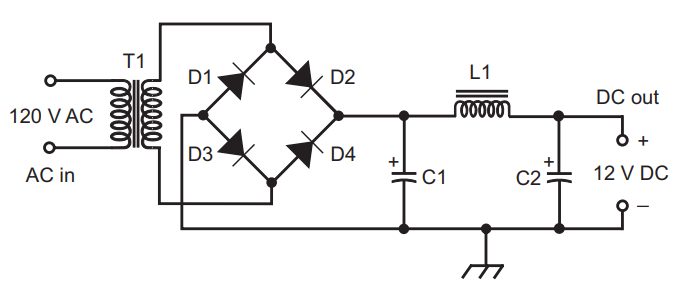
\includegraphics[width=0.5\linewidth]{figuras/Esquematico.png}
    \caption{\textcolor{red}{Diagrama de blocos e esquemático de um circuito conversor de corrente alternada para corrente direta. Extraído de \cite{block_n_schematic}.}}
    \label{fig:diagrama_blocos_e_esquematico}
\end{figure}

\section{Análise de consumo energético}

\subsection{Identificação dos Subsistemas Elétricos}
\label{sec:identificacao_subsistemas}

A identificação dos subsistemas elétricos foi realizada com base nos componentes que consumirão energia durante a operação do micromouse, incluindo sensores, microcontroladores, atuadores, módulos de armazenamento e circuitos de suporte. Para fins de dimensionamento, foi adotado um tempo estimado de uso de 7200\,s, correspondente a uma missão de aproximadamente 2 horas. Os valores de tensão e corrente média foram obtidos a partir de \textit{datasheets} sempre que disponíveis, ou por estimativas conservadoras baseadas em condições realistas de operação.

\begin{table}[htbp]
    \centering
    \caption{Identificação dos subsistemas elétricos e parâmetros de operação}
    \label{tab:subsistemas_eletricos}

    \renewcommand{\arraystretch}{1.2}

    \begin{tabular}{lcccc}
        \hline
        \textbf{Componente} &
        \textbf{Qtde} &
        \textbf{Tensão (V)} &
        \textbf{Corrente média (mA)} &
        \textbf{Tempo (s)} \\
        \hline

        ESP32 & 1 & 3,3 & 200 & 7200 \\
        VL53L0X & 6 & 3,3 & 20 & 7200 \\
        Motor N20 (6V) & 2 & 6,0 & 400 & 7200 \\
        Driver (TB6612) & 1 & 3,3 & 30 & 7200 \\
        MPU6050 & 1 & 3,3 & 4 & 7200 \\
        INA226 & 1 & 3,3 & 0,33 & 7200 \\
        SD Reader & 1 & 3,3 & 80 & 7200 \\
        Regulador (MP1584EN) & 1 & 3,3 & 100 & 7200 \\
        Outros (LEDs, perdas) & -- & 3,3 & 100 & 7200 \\

        \hline
    \end{tabular}
\end{table}

Os valores apresentados na Tabela~\ref{tab:subsistemas_eletricos} contemplam os principais elementos energizados do sistema.

\subsection{Cálculo da Energia Consumida por Componente}
\label{sec:calculo_energia_componente}

A energia consumida por cada componente foi calculada por meio da expressão:

\begin{equation}
E = V \cdot I \cdot t
\end{equation}

em que $E$ representa a energia em joules, $V$ a tensão em volts, $I$ a corrente em ampères e $t$ o tempo de uso em segundos. Para os cálculos, as correntes em miliampères foram convertidas para ampères.

A seguir, apresenta-se o detalhamento da energia consumida por cada subsistema, cujos valores estão sintetizados na Tabela~\ref{tab:energia_por_componente}.

\begin{table}[htbp]
    \centering
    \caption{Energia consumida por componente}
    \label{tab:energia_por_componente}

    \renewcommand{\arraystretch}{1.2}

    \begin{tabular}{lc}
        \hline
        \textbf{Componente} & \textbf{Energia (J)} \\
        \hline

        ESP32 & 4752,00 \\
        VL53L0X & 2851,20 \\
        Motor N20 (2 unidades) & 34560,00 \\
        Driver (TB6612) & 712,80 \\
        MPU6050 & 95,04 \\
        INA226 & 7,84 \\
        SD Reader & 1900,80 \\
        Regulador (MP1584EN) & 2376,00 \\
        Outros (LEDs, perdas) & 2376,00 \\

        \hline
        \textbf{Total} & \textbf{49631,68} \\
        \hline
    \end{tabular}
\end{table}

\subsection{Estimativa do Consumo Total de Energia}
\label{sec:consumo_total_energia}

A energia total estimada por lançamento corresponde à soma das energias individuais dos subsistemas listados anteriormente:

\begin{equation}
E_{\text{total}}
=
4752{,}00 + 2851{,}20 + 34560{,}00 + 712{,}80 + 95{,}04 + 7{,}84 + 1900{,}80 + 2376{,}00 + 2376{,}00
\end{equation}

\begin{equation}
E_{\text{total}}
=
49631{,}68\,\mathrm{J}
\end{equation}

Para expressar esse consumo em watt-hora, utiliza-se a relação:

\begin{equation}
1\,\mathrm{Wh} = 3600\,\mathrm{J}
\end{equation}

Logo, a conversão do consumo total é dada por:

\begin{equation}
E_{\text{total,Wh}}
=
\frac{49631{,}68}{3600}
\approx
13{,}79\,\mathrm{Wh}
\end{equation}

Também é possível estimar a corrente média total do sistema a partir da soma das correntes nominais:

\begin{equation}
I_{\text{nom}}
=
200 + 120 + 800 + 30 + 4 + 0{,}33 + 80 + 100 + 100
=
1434{,}33\,\mathrm{mA}
\end{equation}

Portanto,

\begin{equation}
I_{\text{nom}}
\approx
1{,}434\,\mathrm{A}
\end{equation}

Para tornar o dimensionamento mais robusto, foi aplicada uma margem de segurança de 40\%, a fim de contemplar variações de carga, perdas não modeladas e oscilações durante a operação:

\begin{equation}
I_{\text{proj}}
=
I_{\text{nom}} \times 1{,}4
\end{equation}

Substituindo-se o valor obtido:

\begin{equation}
I_{\text{proj}}
=
1{,}434 \times 1{,}4
\approx
2{,}01\,\mathrm{A}
\end{equation}

Em seguida, considerou-se um fator de utilização de 70\%, uma vez que nem todos os subsistemas operam continuamente em máxima corrente durante toda a missão:

\begin{equation}
I_{\text{real}}
=
I_{\text{proj}} \times 0{,}7
\end{equation}

Assim,

\begin{equation}
I_{\text{real}}
=
2{,}01 \times 0{,}7
\approx
1{,}41\,\mathrm{A}
\end{equation}

A capacidade mínima da bateria pode ser estimada por:

\begin{equation}
C_{\text{min}}
=
I_{\text{real}} \times t
\end{equation}

Para uma autonomia de 2 horas:

\begin{equation}
C_{\text{min}}
=
1{,}41 \times 2
=
2{,}82\,\mathrm{Ah}
\approx
2820\,\mathrm{mAh}
\end{equation}

Para uma autonomia de 3 horas:

\begin{equation}
C_{\text{min}}
=
1{,}41 \times 3
=
4{,}23\,\mathrm{Ah}
\approx
4230\,\mathrm{mAh}
\end{equation}

\subsection{Escolha da Fonte de Alimentação}
\label{sec:escolha_fonte}

Com base no consumo energético total estimado, a demanda por lançamento é de aproximadamente 13,79\,Wh. Considerando uma margem de segurança adicional de 25\%, obtém-se uma demanda projetada de aproximadamente 17,24\,Wh.

\begin{equation}
E_{\text{proj,Wh}}
=
13{,}79 \times 1{,}25
\approx
17{,}24\,\mathrm{Wh}
\end{equation}

A fonte de alimentação selecionada é um conjunto formado por duas células idênticas em série do modelo N21700CG-50 da BAK Battery. Considerando as especificações típicas informadas, cada célula possui tensão nominal de 3,6\,V e capacidade de 5,0\,Ah. Em série, o conjunto passa a fornecer tensão nominal de 7,2\,V, mantendo a capacidade de 5,0\,Ah.

A energia nominal do conjunto é dada por:

\begin{equation}
E_{\text{bat}}
=
7{,}2 \times 5{,}0
=
36\,\mathrm{Wh}
\end{equation}

Esse valor é superior à demanda projetada de 17,24\,Wh, oferecendo folga energética suficiente para o funcionamento do robô.

Como os motores são nominais de 6\,V, o barramento principal será tratado como a alimentação de potência do sistema, enquanto os blocos de lógica, sensores e microcontrolador serão alimentados com tensão regulada pelo MP1584EN para 3,3\,V.

A tabela a seguir resume a escolha da fonte.

\begin{table}[htbp]
    \centering
    \caption{Resumo da fonte de alimentação selecionada}
    \label{tab:fonte_alimentacao}

    \renewcommand{\arraystretch}{1.2}

    \begin{tabular}{lccc}
        \hline
        \textbf{Fonte} & \textbf{Tensão nominal} & \textbf{Capacidade} & \textbf{Energia} \\
        \hline
        2 células em série & 7,2\,V & 5,0\,Ah & 36\,Wh \\
        \hline
    \end{tabular}
\end{table}

subsubsection{Síntese do dimensionamento}

Com base nos cálculos apresentados, o sistema possui consumo energético estimado de 49\,631,68\,J por lançamento, equivalente a aproximadamente 13,79\,Wh. Após aplicação de margem de segurança de 25\%, a demanda projetada passa a ser de aproximadamente 17,24\,Wh.

A fonte selecionada, composta por duas células em série, fornece aproximadamente 36\,Wh, o que atende confortavelmente à demanda do projeto. Dessa forma, a solução escolhida supre a necessidade energética do micromouse e oferece margem adequada para picos de corrente, perdas de conversão e variações operacionais.

Ressalta-se que a corrente dos motores foi considerada em regime nominal de operação, e não em condição de \textit{stall}, evitando superdimensionamento excessivo do sistema de alimentação.

\subsection{Planejamento do Circuito de Alimentação}
\label{sec:planejamento_circuito_alimentacao}

O circuito de alimentação será organizado em dois blocos: potência e lógica. O barramento principal, derivado das duas células em série, alimenta a etapa de potência, enquanto o regulador MP1584EN reduz a tensão para 3,3\,V na etapa lógica.

Para reduzir oscilações de tensão e interferências entre os subsistemas, serão adotadas as seguintes medidas:
\begin{itemize}
    \item uso de regulador buck para a linha de 3,3\,V;
    \item capacitores de desacoplamento próximos aos circuitos integrados;
    \item capacitor de bulk na entrada do sistema;
    \item separação física e elétrica entre alimentação dos motores e da lógica;
    \item uso do driver TB6612 como interface entre ESP32 e motores.
\end{itemize}

A INA226 será utilizada apenas para monitoração de corrente, tensão e potência, permitindo acompanhar o comportamento energético em tempo real. Assim, a estabilidade do sistema será garantida pela combinação entre regulação adequada, desacoplamento e separação das linhas de alimentação.

\section{Referências dos Datasheets}
\label{sec:referencias}

\begin{itemize}

    \item ESP32 -- Espressif Systems. \textit{ESP32 Series Datasheet}. Disponível em:
    \url{https://www.espressif.com/sites/default/files/documentation/esp32_datasheet_en.pdf}

    \item VL53L0X -- STMicroelectronics. \textit{VL53L0X Time-of-Flight Ranging Sensor Datasheet}. Disponível em:
    \url{https://www.st.com/resource/en/datasheet/vl53l0x.pdf}

    \item MPU6050 -- InvenSense. \textit{MPU-6000 and MPU-6050 Product Specification}. Disponível em:
    \url{https://invensense.tdk.com/wp-content/uploads/2015/02/MPU-6000-Datasheet1.pdf}

    \item TB6612FNG -- Toshiba. \textit{TB6612FNG Dual H-Bridge Motor Driver Datasheet}. Disponível em:
    \url{https://toshiba.semicon-storage.com/info/docget.jsp?did=10660}

    \item MP1584EN -- Monolithic Power Systems. \textit{MP1584 3A Step-Down Converter Datasheet}. Disponível em:
    \url{https://www.monolithicpower.com/en/documentview/productdocument/index/version/2/document_type/Datasheet/lang/en/sku/MP1584EN-LF-Z/document_id/221}

    \item INA226 -- Texas Instruments. \textit{INA226 Current/Power Monitor Datasheet}. Disponível em:
    \url{https://www.ti.com/lit/ds/symlink/ina226.pdf}

    \item BAK N21700CG-50 -- BAK Battery. \textit{Product Data Sheet}. Especificações consideradas: tensão nominal de 3,6\,V, capacidade típica de 5,0\,Ah, tensão máxima de carga de 4,2\,V, tensão final de descarga de 2,5\,V, corrente padrão de carga de 0,5C e corrente máxima de descarga de 3C.

    \item Motor N20 6V -- Especificações obtidas a partir do modelo comercial adquirido, complementadas por valores típicos de motores N20 equivalentes utilizados em aplicações embarcadas.

\end{itemize}

\section{Descrição de \textit{software}}

\textcolor{red}{Itens fundamentais:}

\begin{itemize}
    \item \textcolor{red}{ \textbf{Diagrama BPMN para entender o \textit{software} proposto:} deve deixar claro os principais atores do sistema, suas atividades (de negócios), insumos e resultados.}
    \item \textcolor{red}{\textbf{\textit{Backlog} funcional do \textit{software}:}}
    \begin{itemize}
        \item \textcolor{red}{ Escrito no formato de histórias de usuário ou casos de uso (decisão da equipe);}
        \item \textcolor{red}{ Ao declarar o \textit{backlog} de requisitos funcionais, usar a  classificação de MoSCoW (\textit{Must have}, \textit{Should have} e \textit{Could have}),  para um melhor entendimento do próprio \textit{backlog}.}
    \end{itemize}
    \item \textcolor{red}{\textbf{ \textit{Backlog} não-funcional do \textit{software}:}}
    \begin{itemize}
        \item \textcolor{red}{ Descrever os requisitos não-funcionais de forma objetiva;}
        \item \textcolor{red}{ Mais facilmente, mais rapidamente, são descrições subjetivas não-válidas. Um exemplo de requisito não-funcional de desempenho: ``a página deve carregar em até 5s quando em conexão 4G''. }
    \end{itemize}
    \item \textcolor{red}{ \textbf{Diagrama de casos de uso,} contendo os atores do sistema, os requisitos com os quais eles interagem e os tipos de relacionamentos entre requisitos realizados por um mesmo ator (ex.: \textit{include}, \textit{extend}). Obs.: este é um diagrama sobre requisitos funcionais.}
    \item \textcolor{red}{ \textbf{Descrição da arquitetura da solução de \textit{software} proposta:}}
    \begin{itemize}
        \item \textcolor{red}{ Propósito do \textit{software} (qual o seu papel no sistema);}
        \item \textcolor{red}{ Estilo arquitetural contendo:}
        \begin{itemize}
            \item \textcolor{red}{ Padrão adotado: MVC, MVP, Microsserviços, Monolítico, etc (Justificar);}
            \item \textcolor{red}{ Linguagens de programação: Java, Python, C\#, JavaScript, etc.}
            \item \textcolor{red}{ \textit{Frameworks} e bibliotecas: Spring Boot, .NET Core, React, Angular, Django, etc.}
            \item \textcolor{red}{ Banco de dados: Relacional (PostgreSQL, MySQL, etc) X NãoSQL (MongoDB,etc). }
        \end{itemize}
        \item \textcolor{red}{ Diagrama de alto nível: representação esquemática dos componentes da arquitetura, suas responsabilidades e comunicações, esclarecendo a composição do \textit{front-end} e do \textit{back-end}.}
    \end{itemize}
    \item \textcolor{red}{ \textbf{Persistência de dados:} diagrama de entidade relacionamento do banco de dados usado na solução proposta.}
    \item \textcolor{red}{ \textbf{Análise de dados:} as variáveis definidas nos requisitos do projeto em abordagem numérica e gráfica.}
    \item \textcolor{red}{ \textbf{Diagrama de estados} esclarecendo os estados assumidos pelo \textit{software} e os eventos que causam as mudanças de estado do \textit{software}.}
    \item \textcolor{red}{ \textbf{Protótipo funcional do \textit{software}, navegável.}}
    \item \textcolor{red}{\textbf{ Roteiro de testes funcionais:} }
    \begin{itemize}
        \item \textcolor{red}{Código do caso de teste;}
        \item \textcolor{red}{Nome do caso de teste;}
        \item \textcolor{red}{Tipo do caso de teste (unitário, integrado ou sistema);}
        \item \textcolor{red}{ Objetivo do caso de teste;}
        \item \textcolor{red}{ Pré-condições do sistema para o teste ser realizado;}
        \item \textcolor{red}{ Descrição dos procedimentos a serem executados para o teste;}
        \item \textcolor{red}{ Resultado esperado para o teste ser aprovado (pós-condição após realizado o teste);}
        \item \textcolor{red}{ Especificação do reparo a ser executado (caso o teste não seja aprovado);}
        \item \textcolor{red}{ Resultado após reparo (o caso do teste ser necessário de ser repetido após reparo).}
    \end{itemize}
\end{itemize}


% \textcolor{red}{Com relação ao \textit{software}, será necessário apresentar os seguintes itens: % pacotes de componentes de \textit{software}, suas funções e características, e explicar as decisões de projeto:
% \begin{enumerate}
%     \item Um diagrama do processo de negócio do problema que a máquina se propõe a resolver (BPNM) – não é UML, mas é fundamental para entender como o sistema se comporta como um todo, incluindo o usuário;
%     \item Lista de casos de uso (backlog do sistema). Backlog funcional;
%     \item Lista de requisitos não-funcionais a serem satisfeitos pelo sistema;
%     \item Diagrama de casos de uso: mostrando os requisitos funcionais, seus atores e como eles interagem entre si;
%     \item Diagrama de Classes: apresentando quais dados são manipulados pelo sistema (internamente e externamente – ex.: resultados de experimentos);
%     \item Diagrama de arquitetura, identificando todos os componentes da máquina e suas iterações com o software;
%     \item Diagrama de estados da máquina (sistema);
%     \item Descrição dos testes dos componentes da máquina e dos testes funcionais que deveriam ser feitos para avaliar o funcionamento da máquina e identificar defeitos. São importantes os testes unitários (componentes) e de integração (conjunto de componentes) e o roteiro de testes.
% \end{enumerate}
% }
%\textcolor{red}{Com relação ao \textit{software}, será necessário apresentar pacotes de componentes de \textit{software}, suas funções e características, e explicar as decisões de projeto.}
